\documentclass[tikz,border=10pt]{standalone}
\usetikzlibrary{arrows.meta, positioning, fit, backgrounds}
\usepackage{helvet}
\renewcommand{\familydefault}{\sfdefault}

\begin{document}
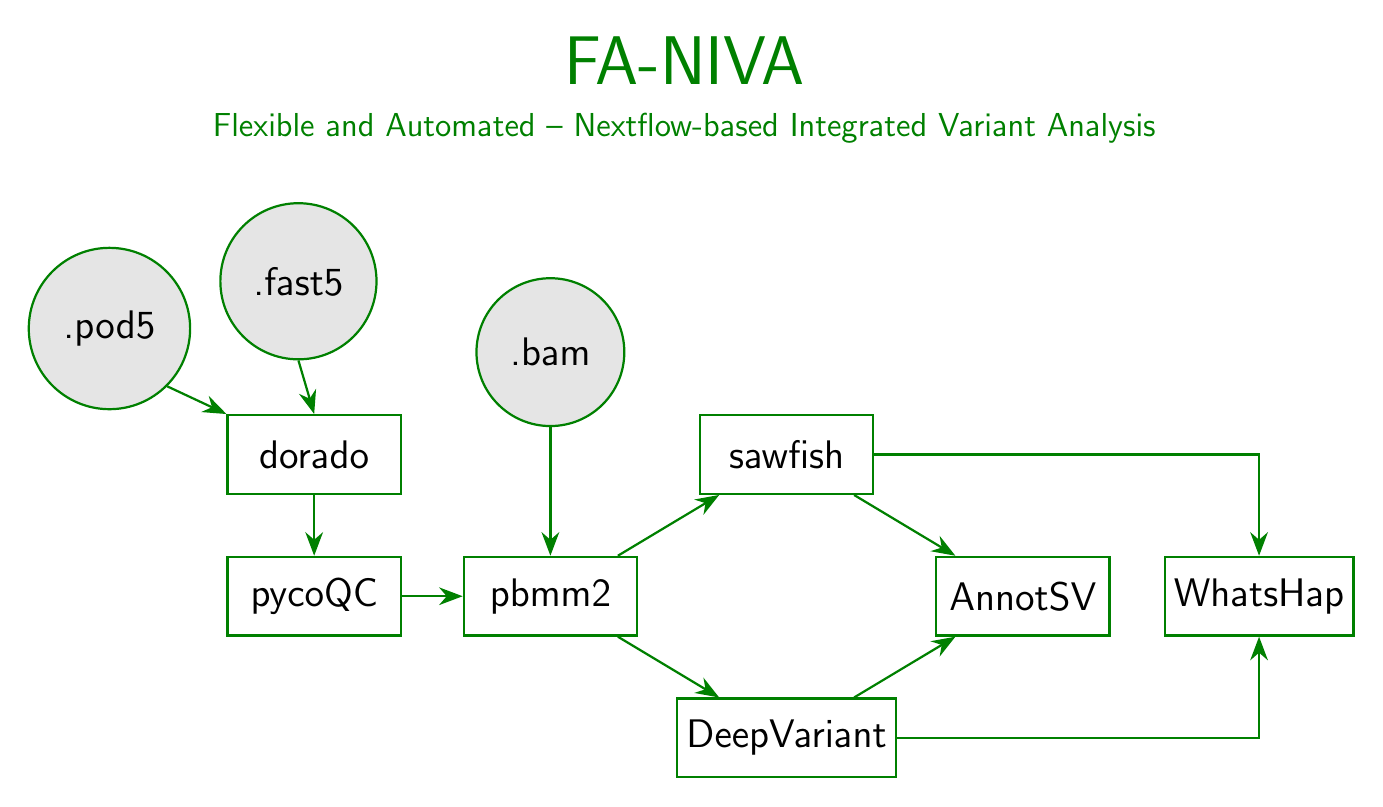
\begin{tikzpicture}[
    >=Stealth,
    node/.style={draw=green!50!black, text=black, thick, minimum width=2.2cm, minimum height=1cm, font=\Large, align=center},
    lbl/.style={text=black, font=\Large, align=center},
    arr/.style={-{Stealth[length=3mm]}, green!50!black, thick},
    circ/.style={draw=green!50!black, fill=gray!20, thick, circle, inner sep=1pt}
]

% ---------- Nodes ----------
\node[node] (dorado)      at (0,6)    {dorado};
\node[node] (pycoqc)      at (0,4.2)  {pycoQC};
\node[node] (pbmm2)       at (3,4.2)  {pbmm2};
\node[node] (sawfish)     at (6,6)    {sawfish};
\node[node] (deepvariant) at (6,2.4)  {DeepVariant};
\node[node] (annotsv)     at (9,4.2)  {AnnotSV};
\node[node] (whatshap)    at (12,4.2) {WhatsHap};

% ---------- Input labels (circled) ----------
\node[lbl] (pod5) at (-2.6,7.6) {.pod5};
\node[lbl] (fast5) at (-0.2,8.2) {.fast5};
\node[lbl] (bam)  at (3,7.3) {.bam};

\begin{scope}[on background layer]
\node[circ, fit=(pod5), inner sep=5pt] (pod5circ) {};
\node[circ, fit=(fast5), inner sep=5pt] (fast5circ) {};
\node[circ, fit=(bam), inner sep=5pt] (bamcirc) {};
\end{scope}

% ---------- Title (centered over whole diagram) ----------
\node[green!50!black, font=\Huge] at (4.7,11) {FA-NIVA};
\node[green!50!black, font=\large] at (4.7,10.15)
    {Flexible and Automated -- Nextflow-based Integrated Variant Analysis};

% ---------- Arrows from inputs (start at circle border) ----------
\draw[arr] (pod5circ.south east) -- (dorado.north west);
\draw[arr] (fast5circ.south) -- (dorado.north);
\draw[arr] (bamcirc.south) -- (pbmm2.north);

% ---------- Main flow ----------
\draw[arr] (dorado) -- (pycoqc);
\draw[arr] (pycoqc) -- (pbmm2);

\draw[arr] (pbmm2) -- (sawfish);
\draw[arr] (pbmm2) -- (deepvariant);

\draw[arr] (sawfish) -- (annotsv);
\draw[arr] (deepvariant) -- (annotsv);

\draw[arr] (sawfish.east) -| (whatshap.north);
\draw[arr] (deepvariant.east) -| (whatshap.south);

\end{tikzpicture}
\end{document}
